% Created by tikzDevice version 0.12.6 on 2025-02-14 03:36:10
% !TEX encoding = UTF-8 Unicode
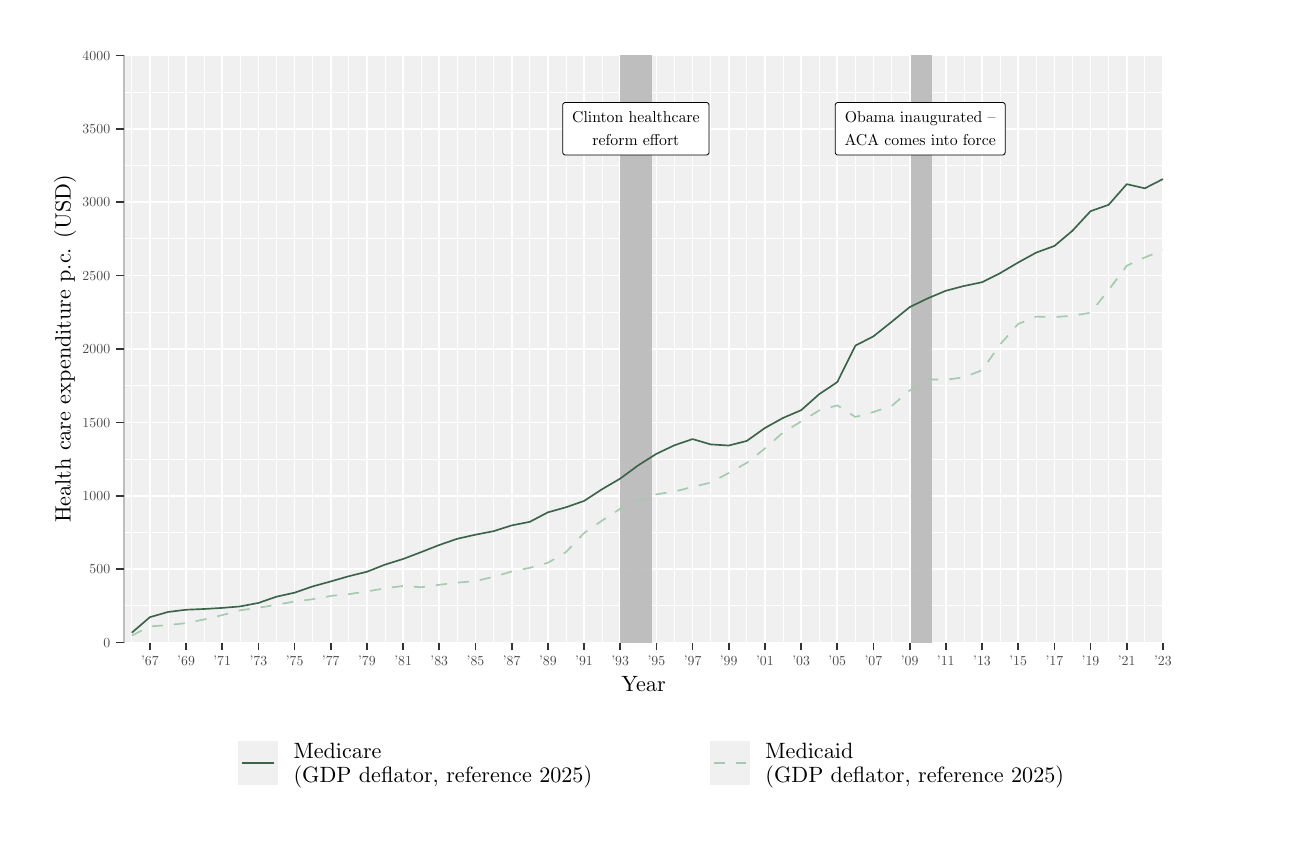
\begin{tikzpicture}[x=1pt,y=1pt]
\definecolor{fillColor}{RGB}{255,255,255}
\path[use as bounding box,fill=fillColor,fill opacity=0.00] (0,0) rectangle (455.30,289.08);
\begin{scope}
\path[clip] (  0.00,  0.00) rectangle (455.30,289.08);
\definecolor{drawColor}{RGB}{255,255,255}
\definecolor{fillColor}{RGB}{255,255,255}

\path[draw=drawColor,line width= 0.6pt,line join=round,line cap=round,fill=fillColor] ( -0.00,  0.00) rectangle (455.30,289.08);
\end{scope}
\begin{scope}
\path[clip] (  0.00,  0.00) rectangle (455.30,289.08);
\definecolor{fillColor}{gray}{0.94}

\path[fill=fillColor] ( 34.76, 66.89) rectangle (410.30,279.08);
\definecolor{drawColor}{RGB}{255,255,255}

\path[draw=drawColor,line width= 0.3pt,line join=round] ( 34.76, 80.15) --
	(410.30, 80.15);

\path[draw=drawColor,line width= 0.3pt,line join=round] ( 34.76,106.67) --
	(410.30,106.67);

\path[draw=drawColor,line width= 0.3pt,line join=round] ( 34.76,133.20) --
	(410.30,133.20);

\path[draw=drawColor,line width= 0.3pt,line join=round] ( 34.76,159.72) --
	(410.30,159.72);

\path[draw=drawColor,line width= 0.3pt,line join=round] ( 34.76,186.24) --
	(410.30,186.24);

\path[draw=drawColor,line width= 0.3pt,line join=round] ( 34.76,212.77) --
	(410.30,212.77);

\path[draw=drawColor,line width= 0.3pt,line join=round] ( 34.76,239.29) --
	(410.30,239.29);

\path[draw=drawColor,line width= 0.3pt,line join=round] ( 34.76,265.82) --
	(410.30,265.82);

\path[draw=drawColor,line width= 0.3pt,line join=round] ( 37.63, 66.89) --
	( 37.63,279.08);

\path[draw=drawColor,line width= 0.3pt,line join=round] ( 50.70, 66.89) --
	( 50.70,279.08);

\path[draw=drawColor,line width= 0.3pt,line join=round] ( 63.77, 66.89) --
	( 63.77,279.08);

\path[draw=drawColor,line width= 0.3pt,line join=round] ( 76.85, 66.89) --
	( 76.85,279.08);

\path[draw=drawColor,line width= 0.3pt,line join=round] ( 89.92, 66.89) --
	( 89.92,279.08);

\path[draw=drawColor,line width= 0.3pt,line join=round] (102.99, 66.89) --
	(102.99,279.08);

\path[draw=drawColor,line width= 0.3pt,line join=round] (116.07, 66.89) --
	(116.07,279.08);

\path[draw=drawColor,line width= 0.3pt,line join=round] (129.14, 66.89) --
	(129.14,279.08);

\path[draw=drawColor,line width= 0.3pt,line join=round] (142.21, 66.89) --
	(142.21,279.08);

\path[draw=drawColor,line width= 0.3pt,line join=round] (155.29, 66.89) --
	(155.29,279.08);

\path[draw=drawColor,line width= 0.3pt,line join=round] (168.36, 66.89) --
	(168.36,279.08);

\path[draw=drawColor,line width= 0.3pt,line join=round] (181.43, 66.89) --
	(181.43,279.08);

\path[draw=drawColor,line width= 0.3pt,line join=round] (194.51, 66.89) --
	(194.51,279.08);

\path[draw=drawColor,line width= 0.3pt,line join=round] (207.58, 66.89) --
	(207.58,279.08);

\path[draw=drawColor,line width= 0.3pt,line join=round] (220.65, 66.89) --
	(220.65,279.08);

\path[draw=drawColor,line width= 0.3pt,line join=round] (233.73, 66.89) --
	(233.73,279.08);

\path[draw=drawColor,line width= 0.3pt,line join=round] (246.80, 66.89) --
	(246.80,279.08);

\path[draw=drawColor,line width= 0.3pt,line join=round] (259.87, 66.89) --
	(259.87,279.08);

\path[draw=drawColor,line width= 0.3pt,line join=round] (272.95, 66.89) --
	(272.95,279.08);

\path[draw=drawColor,line width= 0.3pt,line join=round] (286.02, 66.89) --
	(286.02,279.08);

\path[draw=drawColor,line width= 0.3pt,line join=round] (299.09, 66.89) --
	(299.09,279.08);

\path[draw=drawColor,line width= 0.3pt,line join=round] (312.17, 66.89) --
	(312.17,279.08);

\path[draw=drawColor,line width= 0.3pt,line join=round] (325.24, 66.89) --
	(325.24,279.08);

\path[draw=drawColor,line width= 0.3pt,line join=round] (338.31, 66.89) --
	(338.31,279.08);

\path[draw=drawColor,line width= 0.3pt,line join=round] (351.39, 66.89) --
	(351.39,279.08);

\path[draw=drawColor,line width= 0.3pt,line join=round] (364.46, 66.89) --
	(364.46,279.08);

\path[draw=drawColor,line width= 0.3pt,line join=round] (377.53, 66.89) --
	(377.53,279.08);

\path[draw=drawColor,line width= 0.3pt,line join=round] (390.61, 66.89) --
	(390.61,279.08);

\path[draw=drawColor,line width= 0.3pt,line join=round] (403.68, 66.89) --
	(403.68,279.08);

\path[draw=drawColor,line width= 0.6pt,line join=round] ( 34.76, 66.89) --
	(410.30, 66.89);

\path[draw=drawColor,line width= 0.6pt,line join=round] ( 34.76, 93.41) --
	(410.30, 93.41);

\path[draw=drawColor,line width= 0.6pt,line join=round] ( 34.76,119.93) --
	(410.30,119.93);

\path[draw=drawColor,line width= 0.6pt,line join=round] ( 34.76,146.46) --
	(410.30,146.46);

\path[draw=drawColor,line width= 0.6pt,line join=round] ( 34.76,172.98) --
	(410.30,172.98);

\path[draw=drawColor,line width= 0.6pt,line join=round] ( 34.76,199.51) --
	(410.30,199.51);

\path[draw=drawColor,line width= 0.6pt,line join=round] ( 34.76,226.03) --
	(410.30,226.03);

\path[draw=drawColor,line width= 0.6pt,line join=round] ( 34.76,252.56) --
	(410.30,252.56);

\path[draw=drawColor,line width= 0.6pt,line join=round] ( 34.76,279.08) --
	(410.30,279.08);

\path[draw=drawColor,line width= 0.6pt,line join=round] ( 44.16, 66.89) --
	( 44.16,279.08);

\path[draw=drawColor,line width= 0.6pt,line join=round] ( 57.24, 66.89) --
	( 57.24,279.08);

\path[draw=drawColor,line width= 0.6pt,line join=round] ( 70.30, 66.89) --
	( 70.30,279.08);

\path[draw=drawColor,line width= 0.6pt,line join=round] ( 83.39, 66.89) --
	( 83.39,279.08);

\path[draw=drawColor,line width= 0.6pt,line join=round] ( 96.45, 66.89) --
	( 96.45,279.08);

\path[draw=drawColor,line width= 0.6pt,line join=round] (109.53, 66.89) --
	(109.53,279.08);

\path[draw=drawColor,line width= 0.6pt,line join=round] (122.60, 66.89) --
	(122.60,279.08);

\path[draw=drawColor,line width= 0.6pt,line join=round] (135.68, 66.89) --
	(135.68,279.08);

\path[draw=drawColor,line width= 0.6pt,line join=round] (148.74, 66.89) --
	(148.74,279.08);

\path[draw=drawColor,line width= 0.6pt,line join=round] (161.83, 66.89) --
	(161.83,279.08);

\path[draw=drawColor,line width= 0.6pt,line join=round] (174.89, 66.89) --
	(174.89,279.08);

\path[draw=drawColor,line width= 0.6pt,line join=round] (187.97, 66.89) --
	(187.97,279.08);

\path[draw=drawColor,line width= 0.6pt,line join=round] (201.04, 66.89) --
	(201.04,279.08);

\path[draw=drawColor,line width= 0.6pt,line join=round] (214.12, 66.89) --
	(214.12,279.08);

\path[draw=drawColor,line width= 0.6pt,line join=round] (227.18, 66.89) --
	(227.18,279.08);

\path[draw=drawColor,line width= 0.6pt,line join=round] (240.27, 66.89) --
	(240.27,279.08);

\path[draw=drawColor,line width= 0.6pt,line join=round] (253.33, 66.89) --
	(253.33,279.08);

\path[draw=drawColor,line width= 0.6pt,line join=round] (266.41, 66.89) --
	(266.41,279.08);

\path[draw=drawColor,line width= 0.6pt,line join=round] (279.48, 66.89) --
	(279.48,279.08);

\path[draw=drawColor,line width= 0.6pt,line join=round] (292.56, 66.89) --
	(292.56,279.08);

\path[draw=drawColor,line width= 0.6pt,line join=round] (305.62, 66.89) --
	(305.62,279.08);

\path[draw=drawColor,line width= 0.6pt,line join=round] (318.71, 66.89) --
	(318.71,279.08);

\path[draw=drawColor,line width= 0.6pt,line join=round] (331.77, 66.89) --
	(331.77,279.08);

\path[draw=drawColor,line width= 0.6pt,line join=round] (344.85, 66.89) --
	(344.85,279.08);

\path[draw=drawColor,line width= 0.6pt,line join=round] (357.92, 66.89) --
	(357.92,279.08);

\path[draw=drawColor,line width= 0.6pt,line join=round] (371.00, 66.89) --
	(371.00,279.08);

\path[draw=drawColor,line width= 0.6pt,line join=round] (384.06, 66.89) --
	(384.06,279.08);

\path[draw=drawColor,line width= 0.6pt,line join=round] (397.15, 66.89) --
	(397.15,279.08);

\path[draw=drawColor,line width= 0.6pt,line join=round] (410.21, 66.89) --
	(410.21,279.08);
\definecolor{fillColor}{RGB}{190,190,190}

\path[fill=fillColor,fill opacity=0.01] (214.12, 66.89) rectangle (225.45,279.08);

\path[fill=fillColor,fill opacity=0.01] (214.12, 66.89) rectangle (225.45,279.08);

\path[fill=fillColor,fill opacity=0.01] (214.12, 66.89) rectangle (225.45,279.08);

\path[fill=fillColor,fill opacity=0.01] (214.12, 66.89) rectangle (225.45,279.08);

\path[fill=fillColor,fill opacity=0.01] (214.12, 66.89) rectangle (225.45,279.08);

\path[fill=fillColor,fill opacity=0.01] (214.12, 66.89) rectangle (225.45,279.08);

\path[fill=fillColor,fill opacity=0.01] (214.12, 66.89) rectangle (225.45,279.08);

\path[fill=fillColor,fill opacity=0.01] (214.12, 66.89) rectangle (225.45,279.08);

\path[fill=fillColor,fill opacity=0.01] (214.12, 66.89) rectangle (225.45,279.08);

\path[fill=fillColor,fill opacity=0.01] (214.12, 66.89) rectangle (225.45,279.08);

\path[fill=fillColor,fill opacity=0.01] (214.12, 66.89) rectangle (225.45,279.08);

\path[fill=fillColor,fill opacity=0.01] (214.12, 66.89) rectangle (225.45,279.08);

\path[fill=fillColor,fill opacity=0.01] (214.12, 66.89) rectangle (225.45,279.08);

\path[fill=fillColor,fill opacity=0.01] (214.12, 66.89) rectangle (225.45,279.08);

\path[fill=fillColor,fill opacity=0.01] (214.12, 66.89) rectangle (225.45,279.08);

\path[fill=fillColor,fill opacity=0.01] (214.12, 66.89) rectangle (225.45,279.08);

\path[fill=fillColor,fill opacity=0.01] (214.12, 66.89) rectangle (225.45,279.08);

\path[fill=fillColor,fill opacity=0.01] (214.12, 66.89) rectangle (225.45,279.08);

\path[fill=fillColor,fill opacity=0.01] (214.12, 66.89) rectangle (225.45,279.08);

\path[fill=fillColor,fill opacity=0.01] (214.12, 66.89) rectangle (225.45,279.08);

\path[fill=fillColor,fill opacity=0.01] (214.12, 66.89) rectangle (225.45,279.08);

\path[fill=fillColor,fill opacity=0.01] (214.12, 66.89) rectangle (225.45,279.08);

\path[fill=fillColor,fill opacity=0.01] (214.12, 66.89) rectangle (225.45,279.08);

\path[fill=fillColor,fill opacity=0.01] (214.12, 66.89) rectangle (225.45,279.08);

\path[fill=fillColor,fill opacity=0.01] (214.12, 66.89) rectangle (225.45,279.08);

\path[fill=fillColor,fill opacity=0.01] (214.12, 66.89) rectangle (225.45,279.08);

\path[fill=fillColor,fill opacity=0.01] (214.12, 66.89) rectangle (225.45,279.08);

\path[fill=fillColor,fill opacity=0.01] (214.12, 66.89) rectangle (225.45,279.08);

\path[fill=fillColor,fill opacity=0.01] (214.12, 66.89) rectangle (225.45,279.08);

\path[fill=fillColor,fill opacity=0.01] (214.12, 66.89) rectangle (225.45,279.08);

\path[fill=fillColor,fill opacity=0.01] (214.12, 66.89) rectangle (225.45,279.08);

\path[fill=fillColor,fill opacity=0.01] (214.12, 66.89) rectangle (225.45,279.08);

\path[fill=fillColor,fill opacity=0.01] (214.12, 66.89) rectangle (225.45,279.08);

\path[fill=fillColor,fill opacity=0.01] (214.12, 66.89) rectangle (225.45,279.08);

\path[fill=fillColor,fill opacity=0.01] (214.12, 66.89) rectangle (225.45,279.08);

\path[fill=fillColor,fill opacity=0.01] (214.12, 66.89) rectangle (225.45,279.08);

\path[fill=fillColor,fill opacity=0.01] (214.12, 66.89) rectangle (225.45,279.08);

\path[fill=fillColor,fill opacity=0.01] (214.12, 66.89) rectangle (225.45,279.08);

\path[fill=fillColor,fill opacity=0.01] (214.12, 66.89) rectangle (225.45,279.08);

\path[fill=fillColor,fill opacity=0.01] (214.12, 66.89) rectangle (225.45,279.08);

\path[fill=fillColor,fill opacity=0.01] (214.12, 66.89) rectangle (225.45,279.08);

\path[fill=fillColor,fill opacity=0.01] (214.12, 66.89) rectangle (225.45,279.08);

\path[fill=fillColor,fill opacity=0.01] (214.12, 66.89) rectangle (225.45,279.08);

\path[fill=fillColor,fill opacity=0.01] (214.12, 66.89) rectangle (225.45,279.08);

\path[fill=fillColor,fill opacity=0.01] (214.12, 66.89) rectangle (225.45,279.08);

\path[fill=fillColor,fill opacity=0.01] (214.12, 66.89) rectangle (225.45,279.08);

\path[fill=fillColor,fill opacity=0.01] (214.12, 66.89) rectangle (225.45,279.08);

\path[fill=fillColor,fill opacity=0.01] (214.12, 66.89) rectangle (225.45,279.08);

\path[fill=fillColor,fill opacity=0.01] (214.12, 66.89) rectangle (225.45,279.08);

\path[fill=fillColor,fill opacity=0.01] (214.12, 66.89) rectangle (225.45,279.08);

\path[fill=fillColor,fill opacity=0.01] (214.12, 66.89) rectangle (225.45,279.08);

\path[fill=fillColor,fill opacity=0.01] (214.12, 66.89) rectangle (225.45,279.08);

\path[fill=fillColor,fill opacity=0.01] (214.12, 66.89) rectangle (225.45,279.08);

\path[fill=fillColor,fill opacity=0.01] (214.12, 66.89) rectangle (225.45,279.08);

\path[fill=fillColor,fill opacity=0.01] (214.12, 66.89) rectangle (225.45,279.08);

\path[fill=fillColor,fill opacity=0.01] (214.12, 66.89) rectangle (225.45,279.08);

\path[fill=fillColor,fill opacity=0.01] (214.12, 66.89) rectangle (225.45,279.08);

\path[fill=fillColor,fill opacity=0.01] (214.12, 66.89) rectangle (225.45,279.08);

\path[fill=fillColor,fill opacity=0.01] (214.12, 66.89) rectangle (225.45,279.08);

\path[fill=fillColor,fill opacity=0.01] (214.12, 66.89) rectangle (225.45,279.08);

\path[fill=fillColor,fill opacity=0.01] (214.12, 66.89) rectangle (225.45,279.08);

\path[fill=fillColor,fill opacity=0.01] (214.12, 66.89) rectangle (225.45,279.08);

\path[fill=fillColor,fill opacity=0.01] (214.12, 66.89) rectangle (225.45,279.08);

\path[fill=fillColor,fill opacity=0.01] (214.12, 66.89) rectangle (225.45,279.08);

\path[fill=fillColor,fill opacity=0.01] (319.05, 66.89) rectangle (326.69,279.08);

\path[fill=fillColor,fill opacity=0.01] (319.05, 66.89) rectangle (326.69,279.08);

\path[fill=fillColor,fill opacity=0.01] (319.05, 66.89) rectangle (326.69,279.08);

\path[fill=fillColor,fill opacity=0.01] (319.05, 66.89) rectangle (326.69,279.08);

\path[fill=fillColor,fill opacity=0.01] (319.05, 66.89) rectangle (326.69,279.08);

\path[fill=fillColor,fill opacity=0.01] (319.05, 66.89) rectangle (326.69,279.08);

\path[fill=fillColor,fill opacity=0.01] (319.05, 66.89) rectangle (326.69,279.08);

\path[fill=fillColor,fill opacity=0.01] (319.05, 66.89) rectangle (326.69,279.08);

\path[fill=fillColor,fill opacity=0.01] (319.05, 66.89) rectangle (326.69,279.08);

\path[fill=fillColor,fill opacity=0.01] (319.05, 66.89) rectangle (326.69,279.08);

\path[fill=fillColor,fill opacity=0.01] (319.05, 66.89) rectangle (326.69,279.08);

\path[fill=fillColor,fill opacity=0.01] (319.05, 66.89) rectangle (326.69,279.08);

\path[fill=fillColor,fill opacity=0.01] (319.05, 66.89) rectangle (326.69,279.08);

\path[fill=fillColor,fill opacity=0.01] (319.05, 66.89) rectangle (326.69,279.08);

\path[fill=fillColor,fill opacity=0.01] (319.05, 66.89) rectangle (326.69,279.08);

\path[fill=fillColor,fill opacity=0.01] (319.05, 66.89) rectangle (326.69,279.08);

\path[fill=fillColor,fill opacity=0.01] (319.05, 66.89) rectangle (326.69,279.08);

\path[fill=fillColor,fill opacity=0.01] (319.05, 66.89) rectangle (326.69,279.08);

\path[fill=fillColor,fill opacity=0.01] (319.05, 66.89) rectangle (326.69,279.08);

\path[fill=fillColor,fill opacity=0.01] (319.05, 66.89) rectangle (326.69,279.08);

\path[fill=fillColor,fill opacity=0.01] (319.05, 66.89) rectangle (326.69,279.08);

\path[fill=fillColor,fill opacity=0.01] (319.05, 66.89) rectangle (326.69,279.08);

\path[fill=fillColor,fill opacity=0.01] (319.05, 66.89) rectangle (326.69,279.08);

\path[fill=fillColor,fill opacity=0.01] (319.05, 66.89) rectangle (326.69,279.08);

\path[fill=fillColor,fill opacity=0.01] (319.05, 66.89) rectangle (326.69,279.08);

\path[fill=fillColor,fill opacity=0.01] (319.05, 66.89) rectangle (326.69,279.08);

\path[fill=fillColor,fill opacity=0.01] (319.05, 66.89) rectangle (326.69,279.08);

\path[fill=fillColor,fill opacity=0.01] (319.05, 66.89) rectangle (326.69,279.08);

\path[fill=fillColor,fill opacity=0.01] (319.05, 66.89) rectangle (326.69,279.08);

\path[fill=fillColor,fill opacity=0.01] (319.05, 66.89) rectangle (326.69,279.08);

\path[fill=fillColor,fill opacity=0.01] (319.05, 66.89) rectangle (326.69,279.08);

\path[fill=fillColor,fill opacity=0.01] (319.05, 66.89) rectangle (326.69,279.08);

\path[fill=fillColor,fill opacity=0.01] (319.05, 66.89) rectangle (326.69,279.08);

\path[fill=fillColor,fill opacity=0.01] (319.05, 66.89) rectangle (326.69,279.08);

\path[fill=fillColor,fill opacity=0.01] (319.05, 66.89) rectangle (326.69,279.08);

\path[fill=fillColor,fill opacity=0.01] (319.05, 66.89) rectangle (326.69,279.08);

\path[fill=fillColor,fill opacity=0.01] (319.05, 66.89) rectangle (326.69,279.08);

\path[fill=fillColor,fill opacity=0.01] (319.05, 66.89) rectangle (326.69,279.08);

\path[fill=fillColor,fill opacity=0.01] (319.05, 66.89) rectangle (326.69,279.08);

\path[fill=fillColor,fill opacity=0.01] (319.05, 66.89) rectangle (326.69,279.08);

\path[fill=fillColor,fill opacity=0.01] (319.05, 66.89) rectangle (326.69,279.08);

\path[fill=fillColor,fill opacity=0.01] (319.05, 66.89) rectangle (326.69,279.08);

\path[fill=fillColor,fill opacity=0.01] (319.05, 66.89) rectangle (326.69,279.08);

\path[fill=fillColor,fill opacity=0.01] (319.05, 66.89) rectangle (326.69,279.08);

\path[fill=fillColor,fill opacity=0.01] (319.05, 66.89) rectangle (326.69,279.08);

\path[fill=fillColor,fill opacity=0.01] (319.05, 66.89) rectangle (326.69,279.08);

\path[fill=fillColor,fill opacity=0.01] (319.05, 66.89) rectangle (326.69,279.08);

\path[fill=fillColor,fill opacity=0.01] (319.05, 66.89) rectangle (326.69,279.08);

\path[fill=fillColor,fill opacity=0.01] (319.05, 66.89) rectangle (326.69,279.08);

\path[fill=fillColor,fill opacity=0.01] (319.05, 66.89) rectangle (326.69,279.08);

\path[fill=fillColor,fill opacity=0.01] (319.05, 66.89) rectangle (326.69,279.08);

\path[fill=fillColor,fill opacity=0.01] (319.05, 66.89) rectangle (326.69,279.08);

\path[fill=fillColor,fill opacity=0.01] (319.05, 66.89) rectangle (326.69,279.08);

\path[fill=fillColor,fill opacity=0.01] (319.05, 66.89) rectangle (326.69,279.08);

\path[fill=fillColor,fill opacity=0.01] (319.05, 66.89) rectangle (326.69,279.08);

\path[fill=fillColor,fill opacity=0.01] (319.05, 66.89) rectangle (326.69,279.08);

\path[fill=fillColor,fill opacity=0.01] (319.05, 66.89) rectangle (326.69,279.08);

\path[fill=fillColor,fill opacity=0.01] (319.05, 66.89) rectangle (326.69,279.08);

\path[fill=fillColor,fill opacity=0.01] (319.05, 66.89) rectangle (326.69,279.08);

\path[fill=fillColor,fill opacity=0.01] (319.05, 66.89) rectangle (326.69,279.08);

\path[fill=fillColor,fill opacity=0.01] (319.05, 66.89) rectangle (326.69,279.08);

\path[fill=fillColor,fill opacity=0.01] (319.05, 66.89) rectangle (326.69,279.08);

\path[fill=fillColor,fill opacity=0.01] (319.05, 66.89) rectangle (326.69,279.08);

\path[fill=fillColor,fill opacity=0.01] (319.05, 66.89) rectangle (326.69,279.08);
\definecolor{drawColor}{RGB}{190,190,190}

\path[draw=drawColor,line width= 0.6pt,line join=round] ( 34.85, 66.89) -- ( 34.85,279.08);
\definecolor{drawColor}{RGB}{0,0,0}
\definecolor{fillColor}{RGB}{255,255,255}

\path[draw=drawColor,line width= 0.3pt,line join=round,line cap=round,fill=fillColor] (194.37,243.07) --
	(245.18,243.07) --
	(245.14,243.07) --
	(245.30,243.08) --
	(245.46,243.11) --
	(245.62,243.17) --
	(245.76,243.25) --
	(245.89,243.36) --
	(246.00,243.48) --
	(246.09,243.62) --
	(246.15,243.77) --
	(246.19,243.93) --
	(246.21,244.10) --
	(246.21,244.10) --
	(246.21,261.01) --
	(246.21,261.01) --
	(246.19,261.18) --
	(246.15,261.34) --
	(246.09,261.49) --
	(246.00,261.63) --
	(245.89,261.75) --
	(245.76,261.86) --
	(245.62,261.94) --
	(245.46,262.00) --
	(245.30,262.03) --
	(245.18,262.04) --
	(194.37,262.04) --
	(194.50,262.03) --
	(194.33,262.04) --
	(194.17,262.02) --
	(194.01,261.97) --
	(193.86,261.90) --
	(193.72,261.81) --
	(193.60,261.69) --
	(193.50,261.56) --
	(193.43,261.41) --
	(193.37,261.26) --
	(193.35,261.09) --
	(193.34,261.01) --
	(193.34,244.10) --
	(193.35,244.18) --
	(193.35,244.02) --
	(193.37,243.85) --
	(193.43,243.70) --
	(193.50,243.55) --
	(193.60,243.42) --
	(193.72,243.30) --
	(193.86,243.21) --
	(194.01,243.14) --
	(194.17,243.09) --
	(194.33,243.07) --
	cycle;
\end{scope}
\begin{scope}
\path[clip] (  0.00,  0.00) rectangle (455.30,289.08);
\definecolor{drawColor}{RGB}{0,0,0}

\node[text=drawColor,anchor=base,inner sep=0pt, outer sep=0pt, scale=  0.57] at (219.78,254.69) {Clinton healthcare };

\node[text=drawColor,anchor=base,inner sep=0pt, outer sep=0pt, scale=  0.57] at (219.78,246.50) { reform effort};
\end{scope}
\begin{scope}
\path[clip] (  0.00,  0.00) rectangle (455.30,289.08);
\definecolor{drawColor}{RGB}{0,0,0}
\definecolor{fillColor}{RGB}{255,255,255}

\path[draw=drawColor,line width= 0.3pt,line join=round,line cap=round,fill=fillColor] (292.82,243.07) --
	(352.19,243.07) --
	(352.15,243.07) --
	(352.31,243.08) --
	(352.47,243.11) --
	(352.63,243.17) --
	(352.77,243.25) --
	(352.90,243.36) --
	(353.01,243.48) --
	(353.10,243.62) --
	(353.16,243.77) --
	(353.20,243.93) --
	(353.22,244.10) --
	(353.22,244.10) --
	(353.22,261.01) --
	(353.22,261.01) --
	(353.20,261.18) --
	(353.16,261.34) --
	(353.10,261.49) --
	(353.01,261.63) --
	(352.90,261.75) --
	(352.77,261.86) --
	(352.63,261.94) --
	(352.47,262.00) --
	(352.31,262.03) --
	(352.19,262.04) --
	(292.82,262.04) --
	(292.94,262.03) --
	(292.77,262.04) --
	(292.61,262.02) --
	(292.45,261.97) --
	(292.30,261.90) --
	(292.17,261.81) --
	(292.05,261.69) --
	(291.95,261.56) --
	(291.87,261.41) --
	(291.82,261.26) --
	(291.79,261.09) --
	(291.79,261.01) --
	(291.79,244.10) --
	(291.79,244.18) --
	(291.79,244.02) --
	(291.82,243.85) --
	(291.87,243.70) --
	(291.95,243.55) --
	(292.05,243.42) --
	(292.17,243.30) --
	(292.30,243.21) --
	(292.45,243.14) --
	(292.61,243.09) --
	(292.77,243.07) --
	cycle;
\end{scope}
\begin{scope}
\path[clip] (  0.00,  0.00) rectangle (455.30,289.08);
\definecolor{drawColor}{RGB}{0,0,0}

\node[text=drawColor,anchor=base,inner sep=0pt, outer sep=0pt, scale=  0.57] at (322.50,254.69) {Obama inaugurated -- };

\node[text=drawColor,anchor=base,inner sep=0pt, outer sep=0pt, scale=  0.57] at (322.50,246.50) { ACA comes into force};
\end{scope}
\begin{scope}
\path[clip] (  0.00,  0.00) rectangle (455.30,289.08);
\definecolor{drawColor}{RGB}{60,100,75}

\path[draw=drawColor,line width= 0.6pt,line join=round] ( 37.63, 70.46) --
	( 44.16, 76.06) --
	( 50.69, 77.94) --
	( 57.24, 78.75) --
	( 63.77, 79.02) --
	( 70.30, 79.41) --
	( 76.84, 79.96) --
	( 83.39, 81.21) --
	( 89.92, 83.47) --
	( 96.45, 84.91) --
	(102.98, 87.18) --
	(109.53, 88.98) --
	(116.07, 90.87) --
	(122.60, 92.48) --
	(129.13, 95.06) --
	(135.68, 97.10) --
	(142.21, 99.58) --
	(148.74,102.15) --
	(155.28,104.40) --
	(161.83,105.87) --
	(168.36,107.14) --
	(174.89,109.22) --
	(181.42,110.51) --
	(187.97,113.94) --
	(194.51,115.77) --
	(201.04,118.06) --
	(207.57,122.31) --
	(214.12,126.14) --
	(220.65,130.95) --
	(227.18,135.08) --
	(233.72,138.19) --
	(240.27,140.42) --
	(246.80,138.49) --
	(253.33,138.09) --
	(259.86,139.75) --
	(266.41,144.43) --
	(272.95,148.06) --
	(279.48,150.85) --
	(286.01,156.64) --
	(292.56,161.03) --
	(299.09,174.19) --
	(305.62,177.54) --
	(312.16,182.76) --
	(318.71,188.10) --
	(325.24,191.27) --
	(331.77,194.01) --
	(338.30,195.73) --
	(344.85,197.10) --
	(351.39,200.37) --
	(357.92,204.23) --
	(364.45,207.81) --
	(371.00,210.20) --
	(377.53,215.71) --
	(384.06,222.77) --
	(390.60,225.07) --
	(397.15,232.53) --
	(403.68,231.03) --
	(410.21,234.37);
\definecolor{drawColor}{RGB}{164,203,174}

\path[draw=drawColor,line width= 0.6pt,dash pattern=on 4pt off 4pt ,line join=round] ( 37.63, 69.41) --
	( 44.16, 72.74) --
	( 50.69, 73.18) --
	( 57.24, 73.92) --
	( 63.77, 75.25) --
	( 70.30, 76.81) --
	( 76.84, 78.54) --
	( 83.39, 79.47) --
	( 89.92, 80.57) --
	( 96.45, 81.72) --
	(102.98, 82.54) --
	(109.53, 83.74) --
	(116.07, 84.39) --
	(122.60, 85.37) --
	(129.13, 86.50) --
	(135.68, 87.34) --
	(142.21, 86.88) --
	(148.74, 87.77) --
	(155.28, 88.55) --
	(161.83, 89.10) --
	(168.36, 90.66) --
	(174.89, 92.54) --
	(181.42, 93.90) --
	(187.97, 95.71) --
	(194.51, 99.57) --
	(201.04,106.43) --
	(207.57,110.98) --
	(214.12,115.24) --
	(220.65,118.25) --
	(227.18,120.46) --
	(233.72,121.48) --
	(240.27,123.11) --
	(246.80,124.68) --
	(253.33,128.17) --
	(259.86,131.83) --
	(266.41,137.05) --
	(272.95,142.78) --
	(279.48,146.78) --
	(286.01,150.76) --
	(292.56,152.60) --
	(299.09,148.40) --
	(305.62,150.21) --
	(312.16,152.35) --
	(318.71,157.98) --
	(325.24,162.02) --
	(331.77,161.84) --
	(338.30,162.73) --
	(344.85,165.29) --
	(351.39,174.61) --
	(357.92,182.02) --
	(364.45,184.67) --
	(371.00,184.49) --
	(377.53,185.00) --
	(384.06,186.07) --
	(390.60,194.30) --
	(397.15,203.05) --
	(403.68,206.05) --
	(410.21,208.66);
\end{scope}
\begin{scope}
\path[clip] (  0.00,  0.00) rectangle (455.30,289.08);
\definecolor{drawColor}{gray}{0.30}

\node[text=drawColor,anchor=base east,inner sep=0pt, outer sep=0pt, scale=  0.50] at ( 29.81, 65.16) {0};

\node[text=drawColor,anchor=base east,inner sep=0pt, outer sep=0pt, scale=  0.50] at ( 29.81, 91.69) {500};

\node[text=drawColor,anchor=base east,inner sep=0pt, outer sep=0pt, scale=  0.50] at ( 29.81,118.21) {1000};

\node[text=drawColor,anchor=base east,inner sep=0pt, outer sep=0pt, scale=  0.50] at ( 29.81,144.74) {1500};

\node[text=drawColor,anchor=base east,inner sep=0pt, outer sep=0pt, scale=  0.50] at ( 29.81,171.26) {2000};

\node[text=drawColor,anchor=base east,inner sep=0pt, outer sep=0pt, scale=  0.50] at ( 29.81,197.79) {2500};

\node[text=drawColor,anchor=base east,inner sep=0pt, outer sep=0pt, scale=  0.50] at ( 29.81,224.31) {3000};

\node[text=drawColor,anchor=base east,inner sep=0pt, outer sep=0pt, scale=  0.50] at ( 29.81,250.83) {3500};

\node[text=drawColor,anchor=base east,inner sep=0pt, outer sep=0pt, scale=  0.50] at ( 29.81,277.36) {4000};
\end{scope}
\begin{scope}
\path[clip] (  0.00,  0.00) rectangle (455.30,289.08);
\definecolor{drawColor}{gray}{0.20}

\path[draw=drawColor,line width= 0.6pt,line join=round] ( 32.01, 66.89) --
	( 34.76, 66.89);

\path[draw=drawColor,line width= 0.6pt,line join=round] ( 32.01, 93.41) --
	( 34.76, 93.41);

\path[draw=drawColor,line width= 0.6pt,line join=round] ( 32.01,119.93) --
	( 34.76,119.93);

\path[draw=drawColor,line width= 0.6pt,line join=round] ( 32.01,146.46) --
	( 34.76,146.46);

\path[draw=drawColor,line width= 0.6pt,line join=round] ( 32.01,172.98) --
	( 34.76,172.98);

\path[draw=drawColor,line width= 0.6pt,line join=round] ( 32.01,199.51) --
	( 34.76,199.51);

\path[draw=drawColor,line width= 0.6pt,line join=round] ( 32.01,226.03) --
	( 34.76,226.03);

\path[draw=drawColor,line width= 0.6pt,line join=round] ( 32.01,252.56) --
	( 34.76,252.56);

\path[draw=drawColor,line width= 0.6pt,line join=round] ( 32.01,279.08) --
	( 34.76,279.08);
\end{scope}
\begin{scope}
\path[clip] (  0.00,  0.00) rectangle (455.30,289.08);
\definecolor{drawColor}{gray}{0.20}

\path[draw=drawColor,line width= 0.6pt,line join=round] ( 44.16, 64.14) --
	( 44.16, 66.89);

\path[draw=drawColor,line width= 0.6pt,line join=round] ( 57.24, 64.14) --
	( 57.24, 66.89);

\path[draw=drawColor,line width= 0.6pt,line join=round] ( 70.30, 64.14) --
	( 70.30, 66.89);

\path[draw=drawColor,line width= 0.6pt,line join=round] ( 83.39, 64.14) --
	( 83.39, 66.89);

\path[draw=drawColor,line width= 0.6pt,line join=round] ( 96.45, 64.14) --
	( 96.45, 66.89);

\path[draw=drawColor,line width= 0.6pt,line join=round] (109.53, 64.14) --
	(109.53, 66.89);

\path[draw=drawColor,line width= 0.6pt,line join=round] (122.60, 64.14) --
	(122.60, 66.89);

\path[draw=drawColor,line width= 0.6pt,line join=round] (135.68, 64.14) --
	(135.68, 66.89);

\path[draw=drawColor,line width= 0.6pt,line join=round] (148.74, 64.14) --
	(148.74, 66.89);

\path[draw=drawColor,line width= 0.6pt,line join=round] (161.83, 64.14) --
	(161.83, 66.89);

\path[draw=drawColor,line width= 0.6pt,line join=round] (174.89, 64.14) --
	(174.89, 66.89);

\path[draw=drawColor,line width= 0.6pt,line join=round] (187.97, 64.14) --
	(187.97, 66.89);

\path[draw=drawColor,line width= 0.6pt,line join=round] (201.04, 64.14) --
	(201.04, 66.89);

\path[draw=drawColor,line width= 0.6pt,line join=round] (214.12, 64.14) --
	(214.12, 66.89);

\path[draw=drawColor,line width= 0.6pt,line join=round] (227.18, 64.14) --
	(227.18, 66.89);

\path[draw=drawColor,line width= 0.6pt,line join=round] (240.27, 64.14) --
	(240.27, 66.89);

\path[draw=drawColor,line width= 0.6pt,line join=round] (253.33, 64.14) --
	(253.33, 66.89);

\path[draw=drawColor,line width= 0.6pt,line join=round] (266.41, 64.14) --
	(266.41, 66.89);

\path[draw=drawColor,line width= 0.6pt,line join=round] (279.48, 64.14) --
	(279.48, 66.89);

\path[draw=drawColor,line width= 0.6pt,line join=round] (292.56, 64.14) --
	(292.56, 66.89);

\path[draw=drawColor,line width= 0.6pt,line join=round] (305.62, 64.14) --
	(305.62, 66.89);

\path[draw=drawColor,line width= 0.6pt,line join=round] (318.71, 64.14) --
	(318.71, 66.89);

\path[draw=drawColor,line width= 0.6pt,line join=round] (331.77, 64.14) --
	(331.77, 66.89);

\path[draw=drawColor,line width= 0.6pt,line join=round] (344.85, 64.14) --
	(344.85, 66.89);

\path[draw=drawColor,line width= 0.6pt,line join=round] (357.92, 64.14) --
	(357.92, 66.89);

\path[draw=drawColor,line width= 0.6pt,line join=round] (371.00, 64.14) --
	(371.00, 66.89);

\path[draw=drawColor,line width= 0.6pt,line join=round] (384.06, 64.14) --
	(384.06, 66.89);

\path[draw=drawColor,line width= 0.6pt,line join=round] (397.15, 64.14) --
	(397.15, 66.89);

\path[draw=drawColor,line width= 0.6pt,line join=round] (410.21, 64.14) --
	(410.21, 66.89);
\end{scope}
\begin{scope}
\path[clip] (  0.00,  0.00) rectangle (455.30,289.08);
\definecolor{drawColor}{gray}{0.30}

\node[text=drawColor,anchor=base,inner sep=0pt, outer sep=0pt, scale=  0.50] at ( 44.16, 58.49) {'67};

\node[text=drawColor,anchor=base,inner sep=0pt, outer sep=0pt, scale=  0.50] at ( 57.24, 58.49) {'69};

\node[text=drawColor,anchor=base,inner sep=0pt, outer sep=0pt, scale=  0.50] at ( 70.30, 58.49) {'71};

\node[text=drawColor,anchor=base,inner sep=0pt, outer sep=0pt, scale=  0.50] at ( 83.39, 58.49) {'73};

\node[text=drawColor,anchor=base,inner sep=0pt, outer sep=0pt, scale=  0.50] at ( 96.45, 58.49) {'75};

\node[text=drawColor,anchor=base,inner sep=0pt, outer sep=0pt, scale=  0.50] at (109.53, 58.49) {'77};

\node[text=drawColor,anchor=base,inner sep=0pt, outer sep=0pt, scale=  0.50] at (122.60, 58.49) {'79};

\node[text=drawColor,anchor=base,inner sep=0pt, outer sep=0pt, scale=  0.50] at (135.68, 58.49) {'81};

\node[text=drawColor,anchor=base,inner sep=0pt, outer sep=0pt, scale=  0.50] at (148.74, 58.49) {'83};

\node[text=drawColor,anchor=base,inner sep=0pt, outer sep=0pt, scale=  0.50] at (161.83, 58.49) {'85};

\node[text=drawColor,anchor=base,inner sep=0pt, outer sep=0pt, scale=  0.50] at (174.89, 58.49) {'87};

\node[text=drawColor,anchor=base,inner sep=0pt, outer sep=0pt, scale=  0.50] at (187.97, 58.49) {'89};

\node[text=drawColor,anchor=base,inner sep=0pt, outer sep=0pt, scale=  0.50] at (201.04, 58.49) {'91};

\node[text=drawColor,anchor=base,inner sep=0pt, outer sep=0pt, scale=  0.50] at (214.12, 58.49) {'93};

\node[text=drawColor,anchor=base,inner sep=0pt, outer sep=0pt, scale=  0.50] at (227.18, 58.49) {'95};

\node[text=drawColor,anchor=base,inner sep=0pt, outer sep=0pt, scale=  0.50] at (240.27, 58.49) {'97};

\node[text=drawColor,anchor=base,inner sep=0pt, outer sep=0pt, scale=  0.50] at (253.33, 58.49) {'99};

\node[text=drawColor,anchor=base,inner sep=0pt, outer sep=0pt, scale=  0.50] at (266.41, 58.49) {'01};

\node[text=drawColor,anchor=base,inner sep=0pt, outer sep=0pt, scale=  0.50] at (279.48, 58.49) {'03};

\node[text=drawColor,anchor=base,inner sep=0pt, outer sep=0pt, scale=  0.50] at (292.56, 58.49) {'05};

\node[text=drawColor,anchor=base,inner sep=0pt, outer sep=0pt, scale=  0.50] at (305.62, 58.49) {'07};

\node[text=drawColor,anchor=base,inner sep=0pt, outer sep=0pt, scale=  0.50] at (318.71, 58.49) {'09};

\node[text=drawColor,anchor=base,inner sep=0pt, outer sep=0pt, scale=  0.50] at (331.77, 58.49) {'11};

\node[text=drawColor,anchor=base,inner sep=0pt, outer sep=0pt, scale=  0.50] at (344.85, 58.49) {'13};

\node[text=drawColor,anchor=base,inner sep=0pt, outer sep=0pt, scale=  0.50] at (357.92, 58.49) {'15};

\node[text=drawColor,anchor=base,inner sep=0pt, outer sep=0pt, scale=  0.50] at (371.00, 58.49) {'17};

\node[text=drawColor,anchor=base,inner sep=0pt, outer sep=0pt, scale=  0.50] at (384.06, 58.49) {'19};

\node[text=drawColor,anchor=base,inner sep=0pt, outer sep=0pt, scale=  0.50] at (397.15, 58.49) {'21};

\node[text=drawColor,anchor=base,inner sep=0pt, outer sep=0pt, scale=  0.50] at (410.21, 58.49) {'23};
\end{scope}
\begin{scope}
\path[clip] (  0.00,  0.00) rectangle (455.30,289.08);
\definecolor{drawColor}{RGB}{0,0,0}

\node[text=drawColor,anchor=base,inner sep=0pt, outer sep=0pt, scale=  0.80] at (222.53, 49.26) {Year};
\end{scope}
\begin{scope}
\path[clip] (  0.00,  0.00) rectangle (455.30,289.08);
\definecolor{drawColor}{RGB}{0,0,0}

\node[text=drawColor,rotate= 90.00,anchor=base,inner sep=0pt, outer sep=0pt, scale=  0.80] at ( 15.51,172.98) {Health care expenditure p.c. (USD)};
\end{scope}
\begin{scope}
\path[clip] (  0.00,  0.00) rectangle (455.30,289.08);
\definecolor{fillColor}{RGB}{255,255,255}

\path[fill=fillColor] ( 65.11, 10.00) rectangle (379.95, 36.70);
\end{scope}
\begin{scope}
\path[clip] (  0.00,  0.00) rectangle (455.30,289.08);
\definecolor{fillColor}{gray}{0.94}

\path[fill=fillColor] ( 76.11, 15.50) rectangle ( 90.57, 31.20);
\end{scope}
\begin{scope}
\path[clip] (  0.00,  0.00) rectangle (455.30,289.08);
\definecolor{drawColor}{RGB}{60,100,75}

\path[draw=drawColor,line width= 0.6pt,line join=round] ( 77.56, 23.35) -- ( 89.12, 23.35);
\end{scope}
\begin{scope}
\path[clip] (  0.00,  0.00) rectangle (455.30,289.08);
\definecolor{fillColor}{gray}{0.94}

\path[fill=fillColor] (246.62, 15.50) rectangle (261.08, 31.20);
\end{scope}
\begin{scope}
\path[clip] (  0.00,  0.00) rectangle (455.30,289.08);
\definecolor{drawColor}{RGB}{164,203,174}

\path[draw=drawColor,line width= 0.6pt,dash pattern=on 4pt off 4pt ,line join=round] (248.07, 23.35) -- (259.63, 23.35);
\end{scope}
\begin{scope}
\path[clip] (  0.00,  0.00) rectangle (455.30,289.08);
\definecolor{drawColor}{RGB}{0,0,0}

\node[text=drawColor,anchor=base west,inner sep=0pt, outer sep=0pt, scale=  0.80] at ( 96.07, 24.92) {Medicare };

\node[text=drawColor,anchor=base west,inner sep=0pt, outer sep=0pt, scale=  0.80] at ( 96.07, 16.28) { (GDP deflator, reference 2025)};
\end{scope}
\begin{scope}
\path[clip] (  0.00,  0.00) rectangle (455.30,289.08);
\definecolor{drawColor}{RGB}{0,0,0}

\node[text=drawColor,anchor=base west,inner sep=0pt, outer sep=0pt, scale=  0.80] at (266.58, 24.92) {Medicaid };

\node[text=drawColor,anchor=base west,inner sep=0pt, outer sep=0pt, scale=  0.80] at (266.58, 16.28) { (GDP deflator, reference 2025)};
\end{scope}
\end{tikzpicture}
